\section{Quantum Walk}
We can extend the random walk model to quantum particles. 
They must follow the Schrödinger equation with the Laplacian as Hamiltonian. However, the Schrödinger equation requires that the Laplacian is hermitian; therefore, the network must hold the detailed balance condition \eqref{detail_condition}.
This model is known as “continuos time quantum walk" \cite{Farhi_98, quantum_walk}. This model is used to build quantum algorithms \cite{Quantum_walk_Google, classic_to_quantum_networks}.

Let $G(N,M)$ ba a network. We introduce an Hilbert space $\mathcal{H}$ with an orthonormal basis $\{\ket{i}\}_{i<N}$, where each element $\ket{i}$ indicates their corresponding node $i$, satisfying $\braket{i}{j}=\delta_{ij}$. 
A general general state of the network can be encoded in the ket state $\ket{\psi}$ is define as
\begin{equation}\label{ket_state_quantum}
    \ket{\psi} = \sum_i \sqrt{\rho_i(t)} \ket{i},
\end{equation}
in this way $\rho_i = |\braket{i}{\psi}|^2$ is the projection of the state in the node $i$, in other words the probability that the system can be measured in the node $i$. The norm of $\ket{\psi}$ is normalize to $1$, therefore, the projections $\rho_i$ satisfy the condition $\sum_i \rho_i = 1$.
The Schrödinger equation can be written as
\begin{equation}\label{Schrödinger_quantum_walk}
    \frac{d}{dt}\ket{\psi} = -i\frac{1}{2}\hat L\ket{\psi}.
\end{equation}
where 
\begin{equation}\label{Laplacian_operator}
    \hat L = \sum_{ij} L_{ij}\ket{i}\bra{j}
\end{equation}
is the Laplacian operator.
If we apply a Wick rotation into the equation \eqref{Schrödinger_quantum_walk} we recover the master equation of the classic random walk \eqref{master_eq}.

The solution of the equation \eqref{Schrödinger_quantum_walk} takes the form
\begin{equation}
    \ket{\psi(t)} = \hat U(t,0) \ket{\psi(0)} = e^{-\frac{i}{2}\hat L t} \ket{\psi(0)},
\end{equation}
where $\hat U(t,t') =e^{-\frac{i}{2}\hat L (t-t')}$ is the evolution operator and it is unitary. It holds the following property \begin{equation}
    \hat U(t,t')\hat U(t',t'') = U(t,t'') .
\end{equation}

The quantum walk does not converge to a stationary distribution. 
However, it is possible to define a limiting transition probability for a quantum walk as follow: suppose the system starts at node $\ket{i}$, we measure it after a time $t$, random variable uniformly distributed over the interval $t \in [0,T]$ \cite{quantum_walk}. The transition probability from node $i$ to $j$ is given by
\begin{equation}
    \begin{split}
        \rho_{i\rightarrow j}(T) &= \frac{1}{T}\int_0^T |\bra{i}e^{-i\frac{t}{2}\hat L} \ket{j}|^2 dt\\
        &=\frac{1}{T}\int_0^T \sum_{\lambda,\lambda'}\bra{i}e^{i\frac{t}{2}\hat L}\ket{\lambda}\braket{\lambda}{j} \bra{j}e^{-i\frac{t}{2}\hat L} \ket{\lambda'}\braket{\lambda'}{i} dt\\
        &= \sum_{\lambda,\lambda'}\braket{i}{\lambda}\braket{\lambda}{j}\braket{j}{\lambda'}\braket{\lambda'}{i}\frac{1}{T}\int_0^T e^{-i(\lambda-\lambda')\frac{t}{2}}dt\\
        &= \sum_\lambda|\braket{i}{\lambda}\braket{\lambda}{j}|^2+2\sum_{\lambda\neq\lambda'}\braket{i}{\lambda}\braket{\lambda}{j}\braket{j}{\lambda'}\braket{\lambda'}{j}\frac{1-e^{-i(\lambda-\lambda')\frac{T}{2}}}{i(\lambda-\lambda')T},\\
    \end{split}
\end{equation}
where $\ket{\lambda}$ are the eigenstates of $\hat L$ with eigenvalues $\lambda$. In the limit $T\rightarrow \infty$ it tend to 
\begin{equation}
    \rho_{i\rightarrow j}(T) \xrightarrow[T \rightarrow \infty]{} \sum_\lambda|\braket{i}{\lambda}\braket{\lambda}{j}|^2.
\end{equation}

Let the system be in the state $\ket{\psi}$, also called pure state, we can define the density matrix as
\begin{equation}
    \hat\rho =\ket{\psi}\bra{\psi} = \sum_{ij} \sqrt{\rho_i} \sqrt{\rho_j}\ket{i}\bra{j},
\end{equation}
It is a self-adjoint operator and $\Tr[\hat\rho] = 1$ .

For a generic operator $\hat O(t) = O_{ij}\ket{i}\bra{j}$, the expectation value of the respective observable can be found as \cite{Nielsen_Chuang_2010}
\begin{equation}
        \left< \hat O\right> = \Tr\left[\hat O\hat\rho\right].
\end{equation}
The probability $\rho_k$ to be in the node $k$ can be express using the operator $\hat P_k = \ket{k}\bra{k}$ such that
\begin{equation} \label{state_projection_quantum}
    \begin{split}
        \Tr\left[\hat P_k\hat\rho(t)\right] 
        %= \sum_i \braket{i}{a}\braket{a}{\psi}\braket{\psi}{i}
        %& = \sum_{ijk} \braket{i}{a}\bra{a}\sqrt{\rho_j}\ket{j}\bra{k}\sqrt{\rho_k}\ket{i}\\
        %&= \sum_{ijk} \delta_{i,a}\delta_{a,j}\delta_{k,i}\sqrt{\rho_j}\sqrt{\rho_k}\\
        %= \sqrt{\rho_a}\sqrt{\rho_a} 
        = \rho_k.
    \end{split}
\end{equation}

In the Heisenberg picture, the density operator's evolution can be found solving the different equation called Von Neumann equation
\begin{equation}\label{Von Neumann equation}
    \begin{split}
        \frac{d}{dt}\hat\rho(t) 
        %&= \frac{d}{dt}\left(\ket{\psi(t)}\bra{\psi(t)}\right) = \\
        %&= -\frac{i}{2}\hat L\ket{\psi(t)}\bra{\psi(t)} + \ket{\psi(t)}\bra{\psi(t)}\frac{i}{2}\hat L\\
        &= -\frac{i}{2}\left[\hat L,\rho\right]
    \end{split}
\end{equation}
where $[\cdot,\cdot]$ is the commutator.
The solution of the differential equation is
\begin{equation}
    \hat\rho(t) = \hat U(t,0)\hat\rho(0)\hat U^\dagger(t,0) = e^{-\frac{i}{2}t\hat L}\hat\rho\, e^{\frac{i}{2}t\hat L}.
\end{equation}

Using the cyclic property of the trace and the unity of the evolution operator, it can be proved that the $\Tr[\hat\rho]$ is time invariant.

If the initial distribution over the network is uncertain, we can introduce the density matrix for mixed state. Let be $\{\ket{\psi_k}\}_{k<K\in\mathbb{R}}$ a set of different probability state that can describe the system with probability $p_k$, such that $\sum_k^K p_k = 1$, then the mixed density matrix is define as
\begin{equation}
    \hat \rho = \sum_{k=1}^K p_k \hat \rho_k \qquad \hat\rho_k = \ket{\psi_k}\bra{\psi_k}.
\end{equation}

The temporal evolution of the operator is defined as in eq. \eqref{Von Neumann equation}; the probability to be at node a at time t is the same as in eq. \eqref{state_projection_quantum}. All the properties for the pure state still holds; this can be easily proven using the linearity of the trace.

Using the mixed density matrix we can consider a system that does not start from a defined distribution, but from an ensemble of possible distribution with their probability. 

To study the mixed state we introduce the Von Neumann entropy
\begin{equation}\label{Von_Neumann_entropy}
    S[\hat\rho]=-\Tr[\hat\rho\ln\hat\rho].
\end{equation}
It is the quantum counterpart of the Shannon entropy for classical information theory.
The Von Neumann entropy \eqref{Von_Neumann_entropy} is bounded $0\geq S[\hat\rho] \geq \ln N$. It vanishes for pure states.
The Von Neumann entropy is a time invariance, thus, the evolution operator takes pure state into pure state \cite{Nielsen_Chuang_2010}.


\subsection{1-D Quantum Random Walk}
Consider a toy model: the quantum random walk over a discrete line \cite{Farhi_98}. The probability of moving left or right is $\frac{1}{2}$.
To analyze this model, it is useful to introduce the momentum state $\ket{p}$ such that $\braket{j}{p} = e^{ijp}$, where $-\pi < p< \pi$.

In line the Laplacian is defined as
\begin{equation}
    \hat L \ket{j} = 2\ket{j} -\ket{j-1} -\ket{j+1} . 
\end{equation}
Therefore, applying this to the momentum state
\begin{equation}
    \begin{split}
        \bra{j}\hat L \ket{p} &= \braket{j}{p} -\frac{1}{2}\braket{j-1}{p} -\frac{1}2{}\braket{j+1}{p}\\
        &= e^{ijp} -\frac{1}{2}e^{i(j-1)p} - \frac{1}{2}e^{i(j+1)p}\\
        &= e^{ijp}(\cos(p) - 1) = (\cos(p) - 1)\braket{j}{p}
    \end{split}
\end{equation}

Thus, the amplitude of the walk can be computed as the integral over all the momenta, leading to
\begin{equation}
    \begin{split}
        \bra{j}e^{-i\frac{t}{2}\hat L} \ket{k}&= \frac{1}{2\pi}\int_{-\pi}^{\pi} e^{-i\frac{t}{2}(\cos(p) - 1)} \braket{j}{p} \braket{p}{k} dp\\
        &= \frac{1}{2\pi}\int_{-\pi}^{\pi} e^{-ip(j-k)-i\frac{t}{2}(\cos(p) - 1)}\\
        & = e^{i\frac{t}{2}}(-i)^{k-j}J_{k-j}\left(\frac{t}{2}\right),
   \end{split}
\end{equation}
where $J_{n}(x)$ is the Bessel function of the first kind of order $n$.

Applying the Wick rotation we obtain 
\begin{equation}\label{Bessel_function}
    \left|\bra{j}e^{-i\frac{t}{2}\hat L} \ket{k}\right|^2 = e^{-t} \left(I_{k-j}\left(\frac{t}{2}\right)\right)^2,
\end{equation}
where $I_{n}(x) = i^{n}J_{n}(ix)$ is the modified Bessel function of the first kind.
In the limit $t\gg 1$ it tends to a gaussian centered in the origin and variance $\sqrt{t}$, in accordance with the classical model \cite{mabramowitz64:handbook}.

\subsection{Double tree network}
Another important toy model is the quantum walk on a network consisting of two binary trees of depth $n$ with the ending connected as shown in figure \ref{fig:Double_Tree}.
We start from one root and analyze the probability to reach the other one \cite{quantum_walk}.
Classically, the probability of crossing the network scales exponentially as $2^{-n}$, and it is not computable for big $n$.
However, using the quantum version it remains computable.
\begin{figure}[ht!]
    \centering
    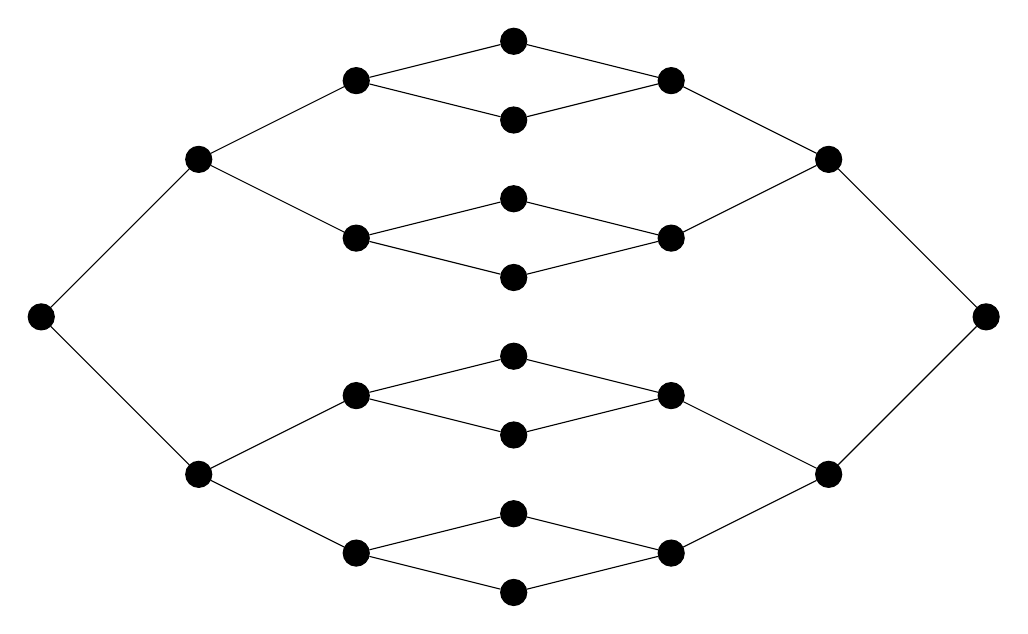
\begin{tikzpicture}[>=stealth, node distance=2cm, every node/.style={circle, draw, fill=black}]
        %draw nodes by coordinates
        \node (n00) at (-6,0) {};
        \node (n11) at (-4,2) {};
        \node (n12) at (-4,-2) {};
        \node (n21) at (-2,3) {};
        \node (n22) at (-2,1) {};
        \node (n23) at (-2,-1) {};
        \node (n24) at (-2,-3) {};
        \node (n31) at (0,3.5) {};
        \node (n32) at (0,2.5) {};
        \node (n33) at (0,1.5) {};
        \node (n34) at (0,0.5) {};
        \node (n35) at (0,-0.5) {};
        \node (n36) at (0,-1.5) {};
        \node (n37) at (0,-2.5) {};
        \node (n38) at (0,-3.5) {};
        \node (n41) at (2,3) {};
        \node (n42) at (2,1) {};
        \node (n43) at (2,-1) {};
        \node (n44) at (2,-3) {};
        \node (n51) at (4,2) {};
        \node (n52) at (4,-2) {};
        \node (n60) at (6,0) {};
        
        % Draw edges (links)
        \draw (n00) -- (n11);
        \draw (n00) -- (n12);
        \draw (n11) -- (n21);
        \draw (n11) -- (n22);
        \draw (n12) -- (n23);
        \draw (n12) -- (n24);
        \draw (n21) -- (n31);
        \draw (n21) -- (n32);
        \draw (n22) -- (n33);
        \draw (n22) -- (n34);
        \draw (n23) -- (n35);
        \draw (n23) -- (n36);
        \draw (n24) -- (n37);
        \draw (n24) -- (n38);
        \draw (n31) -- (n41);
        \draw (n32) -- (n41);
        \draw (n33) -- (n42);
        \draw (n34) -- (n42);
        \draw (n35) -- (n43);
        \draw (n36) -- (n43);
        \draw (n37) -- (n44);
        \draw (n38) -- (n44);
        \draw (n41) -- (n51);
        \draw (n42) -- (n51);
        \draw (n43) -- (n52);
        \draw (n44) -- (n52);
        \draw (n51) -- (n60);
        \draw (n52) -- (n60);
    \end{tikzpicture}
    \caption{The picture of a glued double tree network.}
    \label{fig:Double_Tree}
\end{figure}

To simplify the analysis, we can introduce a new basis $\ket{\mathrm{col}\; j}_{j<2n}$ that indicates a column and not the single node, except at the two root nodes where they coincide. This basis is defined as
\begin{equation}
    \ket{\mathrm{col}\; j} = \frac{1}{\sqrt{N_j}}\sum_{a\in \mathrm{column}} \ket{a}, 
\end{equation}
where the renormalization factor $N_j$ is 
\begin{equation}
    N_j = \left\{\begin{aligned}
        &2^j \qquad &0\leq j\leq n\\
        &2^{2n-j} \qquad &n \leq j \leq 2n
    \end{aligned}\right. .
\end{equation}

In this basis, the Laplacian act as
\begin{equation}
    \begin{aligned}
        \bra{\mathrm{col}\; j}\hat L \ket{\mathrm{col}\; j} &= 1\\
        \bra{\mathrm{col}\; j \pm 1}\hat L \ket{\mathrm{col}\; j} &=\left\{\begin{aligned}
            \frac{\sqrt{2}}{2} \qquad j=0,n,2,\\
            \frac{\sqrt{2}}{3} \qquad \mathrm{otherwise}\\
        \end{aligned}\right.
    \end{aligned}
\end{equation}

Thus, the dynamics along the network reduces to a 1-D quantum walk which has a known computable solution \eqref{Bessel_function} %\cite{quantum_walk}
\begin{equation}
    \bra{0}e^{i\frac{t}{2}\hat L}\ket{2n} = e^{-t} I_{2n}\left(\frac{t}{2}\right),
\end{equation}
where $I_{n}(x) = i^{n}J_{n}(ix)$ is the modified Bessel function of the first kind. 
